\chapter{Function evaluation}

The key purpose of the ScalaAdaptive library is to always invoke a function that is expected to have the best performance possible in given environment and with given inputs. By \textit{function performance} we mean any measurable description of the qualities of the function. It can be the actual run time of the function, memory consumption, number of I/O operations, number of threads created, etc. All these factors can be valuable and be the goal of the system run optimization.

This thesis is focused on the task of optimizing the function run time or time complexity in general. The core of the library, however, is designed to be extensible by modules that can analyze the function run in different ways. More on this topic will be covered in future chapters. %TODO: REFERENCE

\section{Selection and invocation process}
\label{sec:selection_and_invocation_process}

Suppose we have a combined function \inlinecode{f()} created using the API described in chapter \ref{chapter:api} by combining multiple functions \inlinecode{f1()}, ..., \inlinecode{fn()}. We have a new function (or a function-like object) that can be invoked and we expect it to run one of the functions \inlinecode{f1()}, ..., \inlinecode{fn()}.

The basic steps required to do so are the following:

\begin{enumerate}
	\item Locate the history data of \inlinecode{f1()}, ..., \inlinecode{fn()}
	\item Select the function \inlinecode{fk()} to be invoked
	\item Invoke \inlinecode{fk()} and evaluate its run time
	\item Update the history data of \inlinecode{fk()} with the new run time record
\end{enumerate}

\subsection{Run time evaluation}

When talking about function run time (or an execution time of a function), there are two types of values that we could be evaluating:

\begin{itemize}
	\item \textbf{\textit{Wall clock time}} - time elapsed between entering and leaving the function
	\item \textbf{\textit{CPU time}} - time that the CPU actually spent executing our function
\end{itemize}

The \textit{wall clock time} is always higher than the \textit{CPU time}, because it includes not only the time when CPU is executing the function code, but also the time when the executing thread is waiting for its turn in time-sharing multitasking OS or sleeping on a blocking I/O\footnote{Input / Output operation} operation, synchronization primitive, or for some other reason. This means that the \textit{wall clock time} also gets affected by concurrently running processes, network load, and other environment-based factors, and tends to vary much more between multiple invocations.

For the purposes of the ScalaAdaptive library, it might seem that the \textit{CPU time} would be more appropriate, as it gives clearer results not affected by the state of the executing environment. The truth is, however, that many of the use cases of the library require the thread sleeping time to be included in the measurement, as the functions run times are determined mainly by the duration of an I/O operation (e.g. database queries, network requests, etc.), so using \textit{CPU time} wouldn't give us the necessary results.

It is also quite difficult to determine the \textit{CPU time} - it requires support from the executing system with tracking the time that every thread has spent in execution. For this reason and for the reason stated above, the selection process in this text is based on \textit{wall clock time}. It might be, however, interesting as a future extension to implement measuring both of the times and allowing the user to select for each combined function which time should be used.

The \textit{wall clock time} is measured by fetching high-precision system time in nanoseconds right before calling the function apply method and right after returning from the call. The result is the run time in nanoseconds. This measurement is precise enough for all the use cases of the library, because it's targeting mainly functions with non-negligible time complexities.

\subsection{Storing the evaluation data}

After having invoked the function and evaluated its run time, the evaluation data have to be stored before passing the return value back to the caller. The history of all the run time evaluations is kept together for each function as a vector of values. We suppose that multiple combined function that all include one real function will share its run time history. More on that along with different implementation options will be discussed in chapter \ref{chap:implementation}.

\subsection{Selecting a function}

The most complicated task of the entire chain is to select the most appropriate function to run in given case. The case is described by an input $in$ of the function \inlinecode{f()} and by the evaluation data gathered in previous runs. We can use one of various strategies to decide on the result.

The most straightforward approach would be to look at the function run history and select the function with the lowest average runtime in the measured runs. This solution has a few problems. First of all, the runtime of the inner functions \inlinecode{f1()}, ..., \inlinecode{fn()} might depend on the input \inlinecode{in}, which could lead to incorrect assumptions if the historical data were measured on runs with various inputs. And secondly, the method doesn't solve the case where the data don't give us an exact answer, for example if there are too few, if the historical results are too scattered (which might have been caused by different conditions upon invocation, etc.), and in general when we can't make a clear decision and need to collect more data instead.

The \textit{input dependency} problem might be solved in various ways. Methods to analyze the relation between the input and the runtime might be employed in order to predict an approximate runtime on a new input. We call these methods \textit{predictive strategies}. A simpler approach that can be used universally with any \textit{non-predictive strategy} without changing it dramatically is to apply it on a smaller subset of the history records that have inputs of a very similar size. 

As for the \textit{uncertainty} problem, the key is to collect a fixed amount of data first before using any of the strategies. Additionally, a techniques from statistical testing can be used so that the strategy could have a maximal probability of an error (a wrong decision).

Based on these observations, a couple of strategies to select function were proposed and implemented as a part of the ScalaAdaptive library, and will be described in further sections. The user of the library can decide by himself on which one to use.

\section{Predictive strategies}
\label{sec:predictive_strategies}

These strategies are useful solely for the purpose of the functions for which the run time is directly related to the input of the function, e.g. size of a data structure, length of a data file, a number, etc. This relation is usually expressed using the computational complexity of an algorithm, which is a function of the size of the algorithm's input and represents an amount of abstract elementary computational steps that have to be performed. The actual run time depends on the complexity, as every computational step has to take some CPU time. 

The problem is that in reality, the duration of different steps differ as well, depend on hardware optimization, cache misses, pagefaults, scheduling of the OS and many other factors, so the relation, although still present, gets very distorted. In addition, the complexities are often worst-case - the actual complexity can be different for every input as the algorithm execution can vary. Despite these facts and for the purposes of only rough approximation, we will suppose that for function \inlinecode{f()} \(\exists g\) so that 
\(\forall in\) possible inputs holds \(t = g(in)\), where \(t\) is the runtime on input \(in\) of \inlinecode{f()}.

The input, as mentioned earlier, can be a complex structure with a lot of factors contributing to the run time\footnote{Consider for example a general graph - for most of the algorithms, both number of vertices and edges have to be taken into account}. For the simplicity of the strategies, we need to introduce an \textit{input descriptor} - an integer that can be computed from the input and that can be used in the process of finding an approximation of $g$. 

In other words, we suppose that for function \inlinecode{f()} \(\exists h, g_1\) so that
\(g = h \circ g_1\) 
and 
\(\forall in \quad h(in) \in \mathbb{N}\). In this case, the \textit{input descriptor} of input \(in\) would be the value of \(h(in)\).
This assumption is not true in general - we would need at least a multi-dimensional \textit{input descriptor} to cover functions with complexities depending on more factors. In most cases, a sufficient function \(h\) can be found so that the results are precise enough. We call it the \textit{descriptor function}.

The \textit{descriptor function} has to be provided by the user of the library. %TODO: reference to API?
Such function could be:
\begin{itemize}
	\item Number of elements in a data structure argument
	\item Sum of numbers of vertices and edges in a graph
	\item Size of a data file
	\item Identity, if the input is an integer determining the complexity (such as factorial, Fibonacci sequence, etc.)
\end{itemize}
Naturally, the \textit{descriptor function} itself shouldn't have a significant complexity, as it is going to be invoked during every call.

The task of the strategies listed in this section is to make an approximation of the \(g_1\) function and use it to compute \(g_1(h(in))\) upon every invocation and to select the function with the best (minimal) result.

\subsection{Simple linear regression}
\label{subsec:simple_linear_regression}

First strategy supposes that the function \(h\) can be approximated precisely enough using a linear function \(h'\) in the following form:
\[h'(x) = a' x + b'\]

This approximation is a \textit{simple linear regression model}. The slope \(a'\) and intercept \(b'\) of the linear function can be determined using a least squares method, which minimizes the squares of the distances of the actual function values from the ones predicted by the model.

A big advantage of the model is its simplicity and thus minimal overhead when generating the regression during the selection process. 

The main problem is that the linear regression model applied to a case where the relation is not linear leads to a non-trivial errors that increase with the range that we're trying to cover with the model. Figure \ref{fig:selection_sort_linear_trendline} shows samples of run times of the basic selection sort algorithm, which has the complexity of \(O(N^2)\), on sample arrays with 0 to 30000 integers. Collected data obviously match the quadratic function graph marked with the green color. The red line shows the linear regression model. As we can see, the predictions based on this model would be quite inaccurate, especially if we tried to predict run time on an input significantly larger than the samples.

\begin{figure}[h!]
	\centerline{\mbox{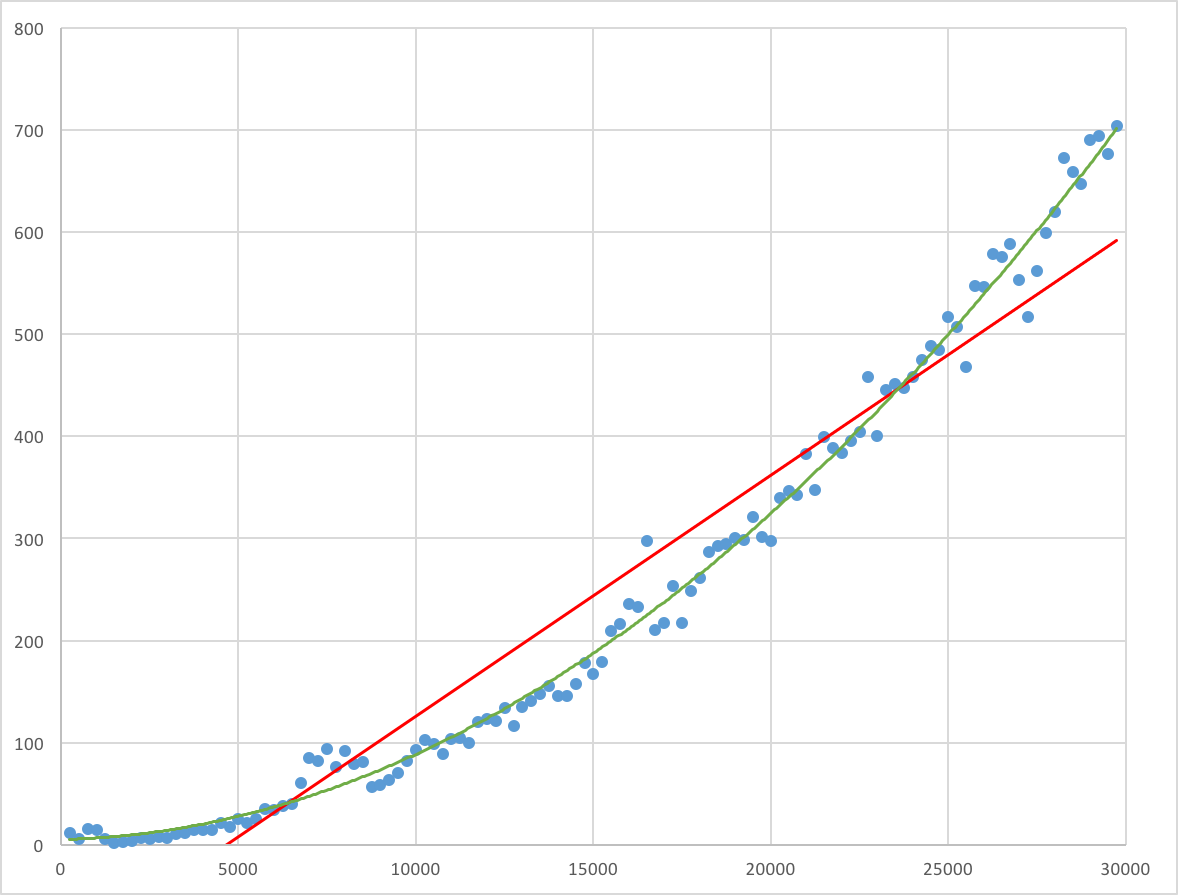
\includegraphics[width=90mm]{./img/selection_sort_linear_trendline.png}}}
	\caption{Linear regression line (red) of a selection sort runtime samples.}
	\label{fig:selection_sort_linear_trendline}
\end{figure}

In order to ensure the accuracy of the model, we can perform statistical tests on it. We can test the true slope \(a\) of the hypothetical original linear function, against a constant value \(a_0\). Suppose we have a linear regression model \(h'(x) = a' x + b'\) constructed using \(n\) data samples \(x_i, y_i\) (in our case, \(x_i\) are the input descriptors and \(y_i\) are the run times). The hypotheses would be the following:

\[H_0: a = a_0\]
\[H_1: a \neq a_0 \]

The test statistics \(T\) for the test can be computed using the following formula:

\[T = \frac{a' - a_0}{se(a')}\]

where

\[se(a') = \sqrt{\frac{\sqrt{MSE}}{ \sqrt{ \sum_{i = 1}^{n} (x_i - \bar{x})^2 }}} \]

and

\[MSE = { \sum_{i = 1}^{n} (y_i - y_i')^2 }\]

The \(\bar{x}\) is the average of \(x_i\) and \(y_i' = h'(x_i)\).

Now, the \(T\) follows a \textit{t-distribution} with \(n-2\) degrees of freedom, so \(H_0\) is rejected on the significance level $\alpha$ in favor of $H_1$ in the following case:

\[\abs{T} > t_{n - 2}(1-\frac{\alpha}{2})\]

The $t_{n - 2}(1-\frac{\alpha}{2})$ is the $(1-\frac{\alpha}{2})$-th quantile of \textit{t-distribution} with $n-2$ degrees of freedom.

In our case, we have no specific $a_0$ that we want to test against, we simply want to know, if the data measured have a linear relation. We can achieve this by putting $a_0 = 0$. If we reject $H_0$ on the significance level $\alpha$, there is a $1 - \alpha$ probability of the data having a linear relation, and in such a situation, we can use the $a'$ slope of the simple linear regression model without too many issues.

\begin{figure}[h!]
	\captionsetup{justification=centering,margin=0.5cm}
	\centerline{\mbox{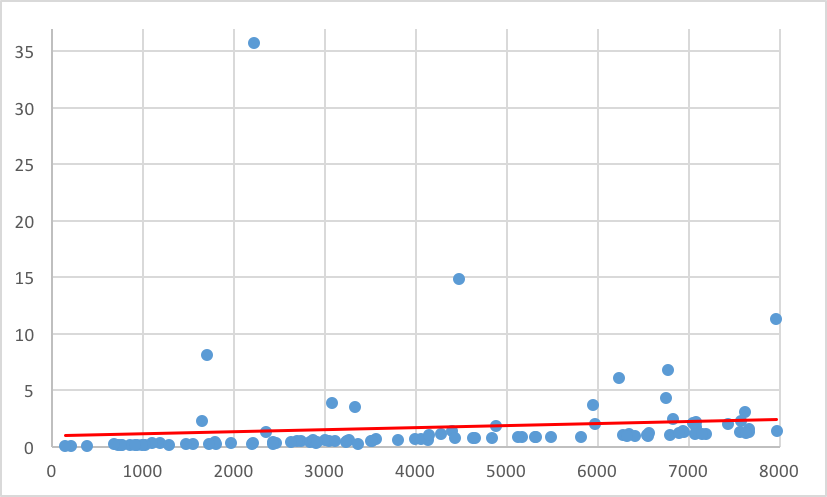
\includegraphics[width=90mm]{./img/linear_cantreject.png}}}
	\caption{Linear regression of 100 run time samples from a function with linear complexity where $H_0$ couldn't be rejected.}
	\label{fig:linear_cantreject}
\end{figure}

Unfortunately, the test tends to get affected by random fluctuations in function run times, which are quite common, especially for simple functions with short execution. The figure \ref{fig:linear_cantreject} shows a regression performed on a sample of 100 run times of a function with linear complexity. The slope of the linear approximation seems to match the measured data reasonably well, but the hypothesis $H_0$ of the statistical test couldn't be rejected on the significance level $\alpha = 0.05$. 

On the other hand, figure \ref{fig:quadratic_rejected} shows a regression performed on a sample of 100 run times of a function with quadratic complexity, and in this case, the hypothesis $H_0$ of the was rejected in favor of $H_1$ on the same significance level $\alpha = 0.05$.

\begin{figure}[h!]
	\captionsetup{justification=centering,margin=0.5cm}
	\centerline{\mbox{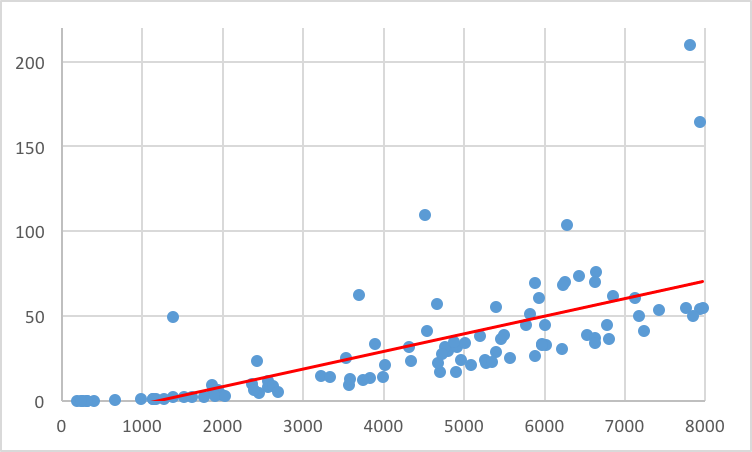
\includegraphics[width=90mm]{./img/quadratic_rejected.png}}}
	\caption{Linear regression of 100 run time samples from a function with quadratic complexity where $H_0$ was rejected.}
	\label{fig:quadratic_rejected}
\end{figure}

\subsection{Window-bound linear regression}
\label{subsec:window_bound_regression}

To be able to apply the strategy described in section \ref{subsec:simple_linear_regression} on a wider range of functions, a simple approach to lower the approximation errors can be taken. Instead of creating a regression model for the entire set of measurements at once, we can split it into more subsets and create different regressions for them. Figure \ref{fig:window_examples} shows ranges $5000 - 10000$, $10000-15000$ and $15000-20000$ of the input sizes of the data from \ref{fig:selection_sort_linear_trendline}. As we can observe from the second and third range, the data tend to be much closer to the linear regression line. The first range shows that a less significant fluctuation in the entire set has a lot bigger impact on a smaller subset.

\begin{figure}[h!]
	\captionsetup{justification=centering,margin=0.5cm}
	\centerline{\mbox{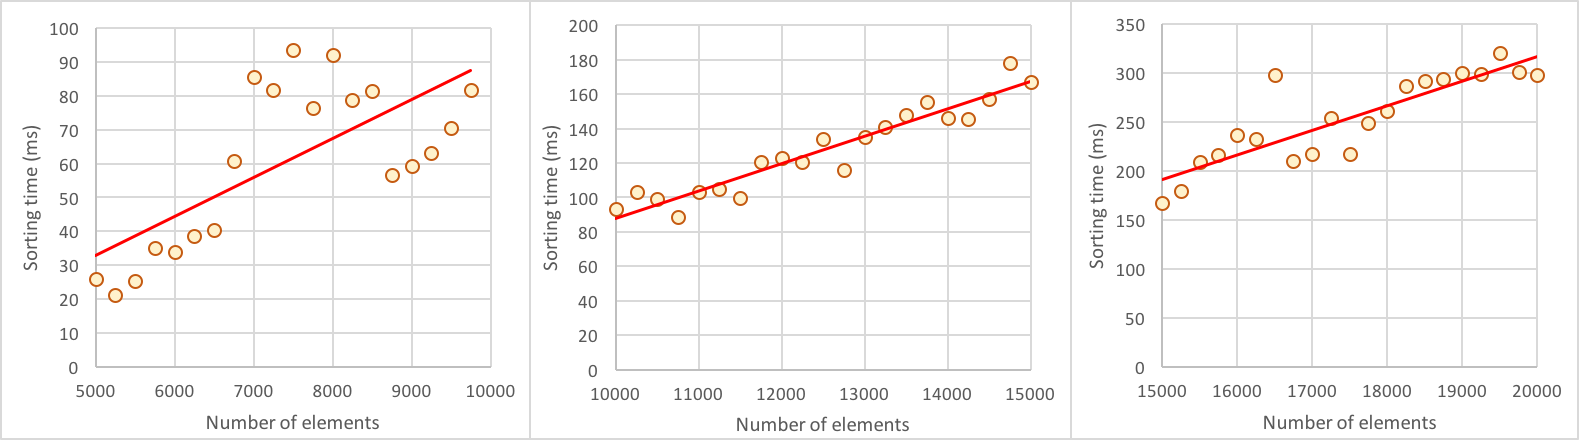
\includegraphics[width=110mm]{./img/window_examples.png}}}
	\caption{Examples of subsets of the data from figure \ref{fig:selection_sort_linear_trendline} with linear regressions.}
	\label{fig:window_examples}
\end{figure}

When selecting a function for a specific \textit{input descriptor} $d$, a window around its value of specific width $w$ can be created and the regression model built upon it. We do it by selecting the data samples $x_k, y_k$ where $\abs{x_k - d} < w$, and using them as the entire data set.

There are multiple ways how to decide on the window width $w$. Using a fixed number across all the functions and all the data samples wouldn't be recommendable, as the functions can vary in their \textit{input descriptors} by orders of magnitude. The width could be derived as a fraction of the width of the whole data set: $w = \frac{max(x_i) - min(x_i)}{p}$, where $p$ would represent in how many parts we basically want to split the set. This wouldn't help us in a case where there are a few extreme values of \textit{input descriptors} in the data set and the rest of the values lie together. 

The most complicated but also the most adaptive window selection method is based on analysis of the entire data set - we sort the samples using the \textit{input descriptor} and compute the distances of each pair of the neighboring ones, make an average of these distances and set the $w$ as $avg * m$, where m is the expected number of samples in one window. For the value of $m$, we can chose a number of about 50-100.

\subsection{Local regression}

The approach explained in \ref{subsec:window_bound_regression} can be extended further - the locally constructed linear regression models can be used to build up a model for the entire data set. This leads to a model that is non-linear, in other words, the function that approximates the original data relation is not a linear function.

One possible regression method that behaves this way is \textit{LOESS} (Local Regression). It uses methods similar to the least-square regression on local subsets of the data set, and then smooths up the resulting curve. The output is a \textit{Loess Curve}, which is a function that is artificially constructed and doesn't have any simple (or even known) formula. This is the one of the advantages - the original relation between \textit{input descriptors} and the run times didn't have to be expressed by a nice simple function in order to be modeled correctly.

%TODO: Add some sources

There is also a few disadvantages of this strategy. First of all, the entire local regression model has to be recomputed whenever there is a new data in the dataset, the model can't be simply updated like the \textit{simple linear regression}. Secondly, it is much more computationally complex and the model construction takes non-trivial time, so it has a negative impact of the library overhead, especially when used with short and simple functions. Next, there is no simple way how to perform statistical tests on the accuracy of the model. The last downside of \textit{local regression} is its inability to predict further behavior past the minimum and maximum data sample.

\subsection{Whitebox model construction}

The methods that were described so far are examples of the blackbox techniques - they don't analyze the function itself, they base all their predictions only on the run time measured.

More thorough predictions could be made after examining the function code as well. It can be analyzed, key structures in the code identified (loops, branches, function calls, variables) and a model can be created using these information. The code can be instrumented and the measurement can be done for each of the structures mentioned. It would require more complex run time measurement data, but the library is prepared for this. The prediction will then be based on the model and the data measured for its elements.

%TODO: Add reference / bibliography
Similar approach was taken in [Predicting Execution Time of Computer Programs] with the goal of predicting program execution time on a specified input with very high precision.
%TODO: Add results?

This approach has a few problems concerning the intended use cases of ScalaAdaptive library. The model won't add any value to the predictions if the majority of the execution time will be spent waiting on an I/O operation. Specifically, it won't help with any of the cases where we are selecting a database query, remote server to connect to, etc.

For these reasons and because of the complexity, it wasn't implemented in the library, but it represents a potential future work that could be done on the topic.

\section{Non-predictive strategies}
\label{sec:non_predictive_strategies}

In some cases, the function run time doesn't depend on the input, or the relation isn't significant enough. In such a situation, we consider all the runs of the function equal and we want to decide based on the historical measurements which one of the functions has a higher chance of being faster.

The trivial solutions being the following:
\begin{itemize}
	\item Select the function with the lowest average run time
	\item Select the function with the lowest minimal run time
	\item Select the function with the lowest maximal run time
\end{itemize}

Each of these strategies does make sense and might be useful in some cases, the problem is that they can't give us the certainty with which the function is better. Again, using statistical methods to express the level of certainty we require from the decision, can solve the problem.

\subsection{T-test for two functions}
\label{subsec:t_test_two}

If we assume that the measured function run times come from a normal distribution, we can use the methods of statistical testing to determine whether one function is faster than the other with given significance. 

Suppose we have two samples of run times for the two functions involved, $X_1, ..., X_n$ and $Y_1, ..., Y_m$. Next, suppose that these samples come from normal distributions with expectations $\mu_1$ and $\mu_2$, respectively. These expectations are unknown for us, just like the variances. The goal is to test the expectations of the two samples against each other. 

Based on these requirements, we will use a \textit{two-sample t-test}. The default hypotheses for the test are:

\[
H_0: \mu_1 = \mu_2
\]
\[
H_1: \mu_1 \ne  \mu_2
\]

and the test statistics

\[
T = \sqrt{\frac{nm}{n + m}}\frac{\bar{X}_n + \bar{Y}_m}{S}
\]

where $\bar{X}_n$ and $\bar{Y}_m$ are the sample means and $S$ is the common variance estimate computed as a weighed average of the sample variances:

\[
S^2 = \frac{1}{n + m -2} ((n-1)S_X^2 + (m-1)S_Y^2)
\]

with $S_X^2$ and $S_Y^2$ being the sample variances:

\[
S_X^2 = \frac{1}{n-1} \sum_{i=1}^{n}(X_i - \bar{X}_n)^2
\]
\[
S_Y^2 = \frac{1}{m-1} \sum_{i=1}^{m}(Y_i - \bar{Y}_m)^2
\]

The hypothesis $H_0$ will be rejected in favor of hypothesis $H_1$ with the significance level $\alpha$ if

\[\abs{T} > t_{n + m - 2}(1-\frac{\alpha}{2})\]

The $t_{n + m - 2}(1-\frac{\alpha}{2})$ is the $(1-\frac{\alpha}{2})$-th quantile of \textit{t-distribution} with $n+m-2$ degrees of freedom.

Rejecting $H_0$ in favor of $H_1$ means that the sample distributions have significantly different expectations, i.e., one of the functions is expected to give better results than the other. In order to find out which of the functions is the favored one, we need to use a \textit{one-sided test}. To do so, we introduce additional hypotheses:

\[
H_2: \mu_1 > \mu_2
\]
\[
H_3: \mu_1 < \mu_2
\]

Now we can reject the hypothesis $H_0$ in favor of $H_2$ if

\[T > t_{n + m - 2}(1-\alpha)\]

or reject the hypothesis $H_0$ in favor of $H_3$ if

\[T < -t_{n + m - 2}(1-\alpha)\]

By performing the \textit{one-sided tests} with $H_2$ and $H_3$ as alternatives, we can easily determine, which of the functions has lower expectation of run time and is a candidate to be selected to run with given certainty (the probability of $1-\alpha$).

\subsection{T-test for multiple functions}
\label{subsec:t_test_multiple}

The selection strategy that was described in \ref{subsec:t_test_two} works only with two functions. If we want to select from three or more, we need to modify the strategy.

The goal of selecting among three or more functions is not as clear as it was for the two functions alternative. Ideally, we would like to be able to identify a function that is significantly better that each one of the remaining functions. The problem is that there might be a function that is significantly better that some of the remaining functions, but not better than all of them. This function can't be selected, because we are not able to rule out the 
possibility that there is a faster option.

For simplicity and possibility to support the decision of the selection strategy with the significance level and the probability connected to it, we will consider only the case where one function is better than all the others. This can, unfortunately, lead to a situation where we have two functions with equally good performance and one with worse performance and we are not able to make a decision.

Suppose we have $k$ samples $X_{1,1}, ..., X_{1, n_1}, ..., X_{k,1}, ..., X_{k, n_k}$ from normal distributions with unknown expectations $\mu_1, ..., \mu_k$ and unknown variances. We would like to compare the expectations and find out whether there is a significant difference or not.

Common techniques for testing hypotheses about the expectations of multiple samples involve \textit{ANOVA}\footnote{Analysis of variance} or its modified version, the \textit{Kruskal-Wallis test}. The tests are based on variance comparison, assume that the samples have similar standard deviations, and can decide about the following hypotheses:

%TODO: Add references to the tests

\[
H_0: \mu_1 = \mu_2 = ... = \mu_k
\]
\[
H_1: \exists i, j: \mu_i \neq \mu_j
\]

These multiple-sample tests are usually preferred over performing multiple t-tests, because in case of the t-tests, it is necessary to correct the significance level by artificially lowering their significance level, which leads to lower test strengths. In our case, however, this approach has a few problems. Firstly, we want to actually find out which of the samples is the deviating one, or, if there are more, which one is the most deviating one. Additionally, we need only one-sided alternative (to find out the lowest expectation). 

Based on these observations, we need to come up with different hypotheses. Lets consider a simple alternative first - suppose we want to test $\mu_1$ against all the other expectations:

\[
H_0: \mu_1 = \mu_2 \vee ... \vee \mu_1 = \mu_k
\]
\[
H_1: \mu_1 < \mu_2 \wedge ... \wedge \mu_1 < \mu_k
\]

$H_0$ is basically saying that there is at least one other sample with the same expectation, and the one-sided alternative $H_1$ puts $\mu_1$ as the lowest of all the expectations.

We can perform a simple t-test of $H_{j,0}: \mu_1 = \mu_j$ against $H_{j,1}: \mu_1 < \mu_j$ $\forall j = 2, ..., k$. It is clear that the $H_0$ can be rejected in favor of $H_1$ only if all of the $H_{j,0}$ were rejected in favor of $H_{j,1}$. 

As mentioned before, the procedure of combining statistical tests usually requires to artificially lower the significance level of the individual tests with the goal of keeping the significance level of the whole set of tests reasonably low. These methods are based on the assumption that committing a type-I error in any of the individual tests leads to a type-I error overall, and the probability of committing at least one gets higher with the number of tests.

In our case, however, a type-I error in one of the individual tests doesn't necessarily lead to a type-I error in the whole test. Suppose that $H_0$ is true, so for an $l \geq 1$ $\exists i_1,...,i_l: \mu_1 = \mu_{i_1} \wedge ... \wedge \mu_1 = \mu_{i_l}$. In order to commit a type-I error, we need to reject $H_{i_j,0}$ $\forall j = 1, ..., l$, thus committing the type-I error on the individual tests $l$-times. At the same time, we need to decide correctly about the remaining $k-l$ tests. So the probability of committing a type-I error overall is $\alpha^l(1-\alpha)^{k-l}$, and consequentially, the significance level of the entire test gets even lower than $\alpha$. The assumption is that the number $k$ of the functions involved will be low enough not to affect the significance too much.

Now, we are able to decide about a function whether it's significantly better than all of the others. In the selection strategy, this test will be performed for all the functions one by one and the first one where the $H_0$ is rejected in favor of $H_1$ gets selected. This means performing at most $k$ of these combined tests. In this case, the type-I error in any of the tests leads to a critical error of the selection process and we should try to keep it as unlikely as possible, by applying one of the correction techniques mentioned. A simple example of such a technique could be the \textit{Bonferroni correction}, which sets the $\alpha'$ of the individual tests to $\alpha / k$ for $\alpha$ being the desired significance overall and $k$ the number of samples.

\subsection{Window-bound t-test}

The t-test methods as described in this section work with all the run data collected and use it to make a decision about the function with the best performance. It works under the assumption that the run times of a specific function have a normal distribution. This could be the truth only for the functions with constant complexity - whenever the function run time depends on the input, the distribution of the sample of measurements depends heavily on the distribution of the inputs.

Even if we assumed that the inputs were distributed normally and that the relation was linear, the whole procedure could only decide about the better function overall, which might not be desirable in the cases where we want to select different function for different inputs based on their size or other factors (in the way the predictive strategies work).

\begin{figure}[h!]
	\centerline{\mbox{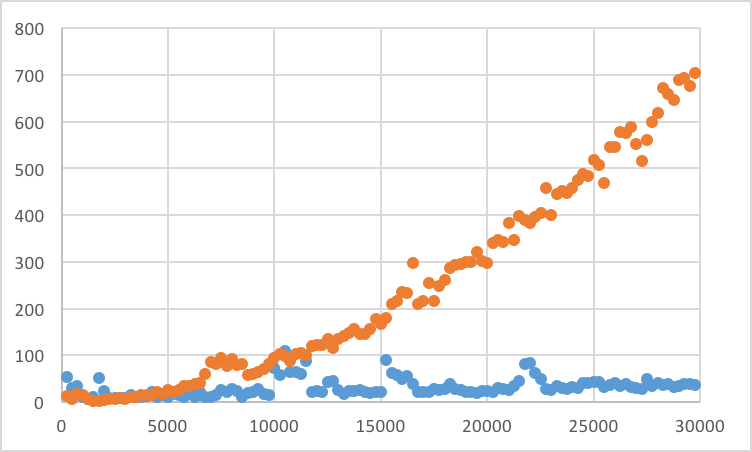
\includegraphics[width=90mm]{./img/quick_vs_selection.png}}}
	\caption{Run times of quick sort algorithm (blue dots) and selection sort algorithm (red dots) by input size.}
	\label{fig:quick_vs_selection}
\end{figure}

\begin{figure}[h!]
	\centerline{\mbox{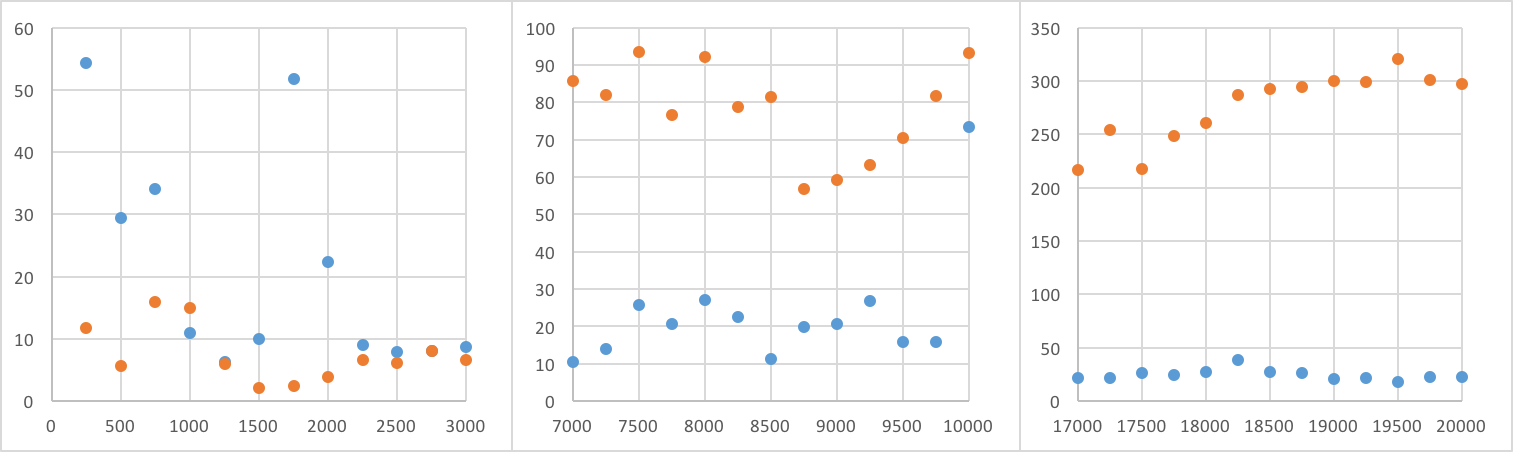
\includegraphics[width=110mm]{./img/window_t_test_examples.png}}}
	\caption{Examples of subsets of the data from figure \ref{fig:quick_vs_selection}}
	\label{fig:window_t_test_examples}
\end{figure}

If we wanted to use the t-test strategy on the functions with non-constant complexity, the same approach as with the \textit{simple linear regression} can be taken - we can perform the t-test just for a subset of the historical data with very similar \textit{input descriptors}. Instead of assuming that the relation in the small window is linear, we want it to be constant and normally distributed. Consequently, even smaller window sizes should be selected, so that these assumptions held at least approximately. The t-test significance levels and strengths will be approximate as well, but our goal is to get reasonable results, we don't need to be precise.

The figure \ref{fig:quick_vs_selection} shows the run times measured for a quick sort and selection sort algorithms. Obviously, there is a relation to the input size, so the simple t-test wouldn't help us in this case. In figure \ref{fig:window_t_test_examples}, there are the same data in three different windows - 0-3000, 7000-10000 and 17000-20000. As we can see, in a window of this size, the run times are almost constant and the random fluctuations are more significant than the actual relation to the input size. We can apply the t-test as described in sections \ref{subsec:t_test_two} and \ref{subsec:t_test_multiple} to these windows and use the result as relevant enough with respect to the input.

If we reduce the window size to a constant 0, we will get a method in which only the results for inputs with the same descriptor are tested. This might be useful in cases where we know that the function will be called 

\section{Strategy comparison}

The predictive strategies don't handle well more historical results for the same \textit{input descriptor}.

\begin{itemize}
	\item \textbf{Dependency on the input} \\
	If the function doesn't have any input, or the input doesn't affect the expected run time (the complexity is constant), non-predictive strategies should be used.
	\item \textbf{Expected input values} \\
	If the function is expected to be invoked with a discrete and very limited set of inputs, non-predictive strategy is preferred. On the other hand, if the function will be called repeatedly with randomly distributed inputs, the predictive strategies are a better choice.
\end{itemize}

\section{Selection policies}

The selection process and all the strategies described in sections \ref{sec:predictive_strategies} and \ref{sec:non_predictive_strategies} are quite complex and have non-trivial overhead, especially after collecting a large amount of historical data. In a common scenario where we expect the system to come to a decision about the best function (either overall, or for every group of \textit{input descriptors}), it would be handy if we could stop the selection process at a certain point and keep using only the most favored function with no extra overhead. Or, to use it most of the time, with only occasional attempts at the selection in order to detect possible changes in the system (response times, I/O operation duration, etc.).

Similarly, it might be desirable to control the overhead time spent on the selection, or, in general, on invoking the functions using selection (which might lead to a bad decision), either per a specific time period, or per a specific action of the system (user request, processing unit, etc.). All of these decisions are taken at a higher level than the run time history analysis performed by the selection strategies.  

\textit{Selection policies} are a concept introduced into the ScalaAdaptive library that tries to address these cases, with the main purpose of lowering its execution overhead. Every \textit{combined function} has a \textit{selection policy} associated with it. In the function selection chain, the \textit{policy} gets evaluated right after invoking the \textit{combined function} and is supposed to quickly decide how to proceed with the invocation. There might be scenarios where a faster ways could be taken without even using any of the strategies and analyzing the historical data.

The possible results of the \textit{policy} evaluation are the following:

\begin{itemize}
	\item \textbf{SelectNew} - Select function using the selection strategy, executing the chain described in section \ref{sec:selection_and_invocation_process}
	\item \textbf{GatherData} - Gather more data for the least-executed function (function selection is skipped, but the run time is measured and the data is stored to the history)
	\item \textbf{UseLast} - Use the function selected last time (without measuring run time and storing it to the history)
	\item \textbf{UseMost} - Use the most selected function (without measuring run time and storing it to the history)
\end{itemize}

We can notice that these results require only the basic statistical data about previous selection processes. This is the key idea of the \textit{policies} - the decision and the execution should depend only on these simple statistics, except for the case where selection strategy is required.

The \textit{policy} evaluation process also replaces the current \textit{policy} with a new one. This technically creates a state machine - the state of the function is represented by the active \textit{policy}, and whenever the function is invoked, a result is produced and new \textit{policy} becomes active. This corresponds to producing output and moving to a new state in a state machine.

The advantage of the \textit{policy} system over a regular state machine is its extensibility and reusability - there are no rules directly in the state machine (i.e. here in the \textit{combined function}). All the logic of deciding on the result and the next \textit{policy} is in the \textit{policy} node itself. So the entire behavior of the state machine is defined by the initial \textit{policy}, which should be specified by the user upon creating the \textit{combined function}. As a result, reusable policies that are parametrized can be used in various chains of policies, smaller chains can be put together, etc.
%TODO: Reference to the API

\subsection{Statistical data}
\label{subsec:statistical_data}

The only input that the \textit{policy} receives when making decision is a statistical summary of previous selection results of the \textit{combined function}. The process itself is supposed to be fast and reflect just the trends in the selection, not to replace the whole selection strategy process as described in sections \ref{sec:predictive_strategies} and \ref{sec:non_predictive_strategies}, so the statistical data don't contain the entire run history of all the functions involved.

\begin{figure}[h!]
	\captionsetup{justification=centering,margin=0.5cm}
	\centerline{\mbox{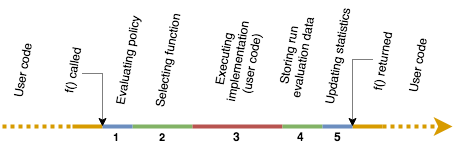
\includegraphics[width=110mm]{./img/run_schema.png}}}
	\caption{Process of \textit{combined function} invocation.}
	\label{fig:run_schema}
\end{figure}

On the other hand, the \textit{policies} are a handy tool to limit the damage of the selection process on the system. For this, it is necessary to observe and to store various times connected with the selection and execution. Figure \ref{fig:run_schema} shows the whole process with policy being evaluated with the SelectNew result, split into individual parts. Upon every invocation, the following is tracked:

\begin{itemize}
	\item Selection and run history storage time (2 and 4)
	\item Function execution time (3)
	\item Total time spent on the SelectNew result (2, 3 and 4)
	\item Total time spent on the GatherData result (3 and 4, 2 is skipped in such a case)
\end{itemize}

Sums of these times are kept in every \textit{combined function}. The policy can work with these totals and analyze the changes that happen to them overtime. The policies are designed to be immutable, but contain state themselves, and the state changes when switching to a new policy.

In addition, number of times each function was selected, total number of times we received the SelectNew and GatherData result and the total number of times the combined function was invoked has to be tracked. The user-implemented policy has the following data available to decide:

\begin{itemize}
	\item Total run count of the combined function
	\item Total number of times the last function was selected
	\item Total number of times the most selected function was selected
	\item Total number of times any function was selected
	\item Total number of times of gathering new data (GatherData result)
	\item Total time spent on function execution (after SelectNew result)
	\item Total time spent on selection and storage overhead (after SelectNew result)
	\item Total time spent on processing the SelectNew result
	\item Total time spent on processing the GatherData result
\end{itemize}

\subsection{Implemented policies}

As mentioned earlier, \textit{policies} are designed to be reusable as a building-blocks. The immutable \textit{policy} itself is the only holder of the state and change of state can be performed only by transitioning to a different \textit{policy}. Its functionality and very simple decision-making process can be visualized using a transition diagram, which shows the \textit{policy} itself as a red square, all the other \textit{policies} as a gray square and green arrows as state transitions. The transitions might be conditional, in such a case, the condition splits the arrow into two. The transition can produce a result which is shown next to the transition arrow. If a result is produced, the \textit{policy} makes a decision and next \textit{policy} will be evaluated during the following invocation. If a result isn't produced, the \textit{policy} just delegates the decision to the next \textit{policy} which is evaluated immediately. The chain of evaluation stops when a result is produced.

The transition conditions use \textit{policy} parameters, which are passed to a \textit{policy} in the constructor, and the current statistic data explained in section \ref{subsec:statistical_data}. It can also use static data and methods that it has access to. The parameters of the top-level (starting) \textit{policy} are passed in by the user creating it, the parameters of the other policies in the chain are fixed when the \textit{policies} are created, usually during the decision of the top-level \textit{policy}, which typically builds the entire policy chain (that can be cyclic and lead back to it).

The transition diagrams and short descriptions of some \textit{policies} will follow.

\subsubsection{Building blocks}

\begin{figure}[h!]
	\centerline{\mbox{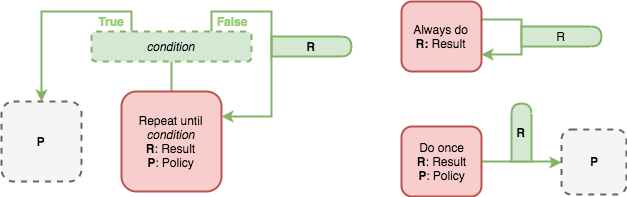
\includegraphics[width=110mm]{./img/helper_policies.png}}}
	\caption{Transition diagram of the basic building-block policies.}
	\label{fig:helper_policies}
\end{figure}

Figure \ref{fig:helper_policies} shows the main policies that serve as a building-blocks. The most important is the \textbf{Repeat until \textit{condition}} \textit{policy}, parametrized by a \textit{condition}, result \textit{R}, which it keeps producing until the \textit{condition} becomes true, and the policy \textit{P}, which it makes transition to at that moment. The \textbf{Always do} \textit{policy} represents an infinite loop producing the same result \textit{R} every time, and the \textbf{Do once} \textit{policy} produces the result \textit{R} once and immediately makes transition to the policy \textit{P}.

\begin{figure}[h!]
	\centerline{\mbox{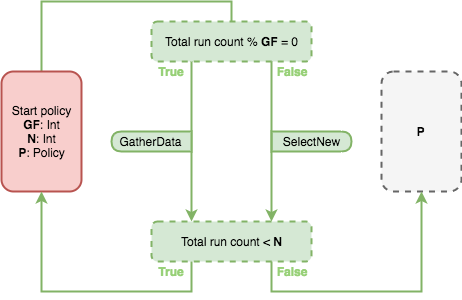
\includegraphics[width=75mm]{./img/start_policy.png}}}
	\caption{Transition diagram of the \textbf{Start policy}.}
	\label{fig:start_policy}
\end{figure}

Figure \ref{fig:start_policy} represents the \textbf{Start policy}, which accepts the gather frequency \textit{GF}, number of invocation times before moving to a next policy \textit{N}, and the policy itself \textit{P}. It's a little more complicated and specialized version of the \textbf{Repeat until} policy - it keeps producing the SelectNew result, and every \textit{GF}-th invocation, it produces the GatherData result. It might be useful at the beginning, when it's necessary to gather data for all of the functions and perform some selections so that the following policies had statistical data to base their decision on.

\subsubsection{Stop selecting when decided}

\begin{figure}[h!]
	\centerline{\mbox{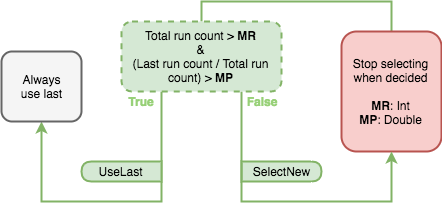
\includegraphics[width=75mm]{./img/stop_selecting_when_decided.png}}}
	\caption{Transition diagram of the \textbf{Stop selecting  when decided} policy.}
	\label{fig:stop_selecting_when_decided}
\end{figure}

In order to limit the overhead, it might be useful to completely stop selecting when we are sure that one of the functions gets selected a lot more often. The \textbf{Stop selecting when decided} policy shown in figure \ref{fig:stop_selecting_when_decided} keeps selecting new function until both the total number of invocations exceeds minimum run count \textit{MR} and the rate of the number of times that the last selected function was selected and the total number of invocations exceeds the minimum percentage \textit{MP}. After that, it will keep using the last function forever. 

The advantage of falling back to the infinite \textbf{Always use last} policy is its basically zero overhead - no condition is evaluated in the decision process. So this policy is useful for the fast functions where keeping low overhead for the long-term is critical. It can't however, undo a wrong decision, reflect a change in conditions, or anything else.

\subsubsection{Pause selection after streak}

\begin{figure}[h!]
	\centerline{\mbox{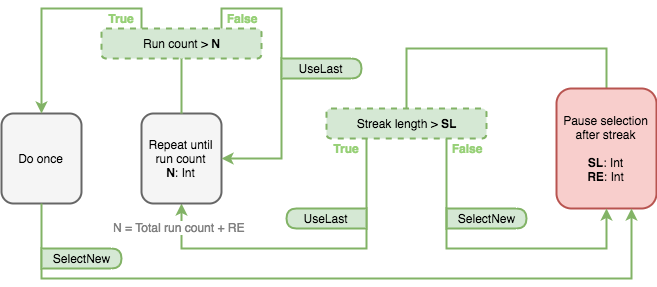
\includegraphics[width=85mm]{./img/pause_selection_after_streak.png}}}
	\caption{Transition diagram of the \textbf{Pause selection after streak} policy.}
	\label{fig:pause_selection_after_streak}
\end{figure}

To lower the number of selections, an approach based on the streak lengths can be used as well. It is implemented by the \textbf{Pause selection after streak} policy in figure \ref{fig:pause_selection_after_streak}. Its functionality is defined by the \textit{SL} (streak length) and \textit{RE} (retry every) arguments. Whenever one function is selected \textit{SL} times in a row, the selection process stops and the UseLast result is being produced. Once every \textit{RE} times, a new selection attempt is done, looping back to the original policy. If the same function is selected once again, the streak gets longer by one and the selection process stops again. If, however, a different function is selected this time, the streak becomes zero and we start selecting again.

The described behavior is the preferred way of limiting the selection overhead. By setting the streak length to a reasonable number (20-100, based on the data, situation, etc.), we can assure that if one function is significantly better than the others, it will be used without the need to select it. The retry that happens every once in a while makes sure that eventual wrong decision will be detected and will reset the system back to the beginning.

\subsubsection{Limited overhead, gather time and selection time}

\begin{figure}[h!]
	\centerline{\mbox{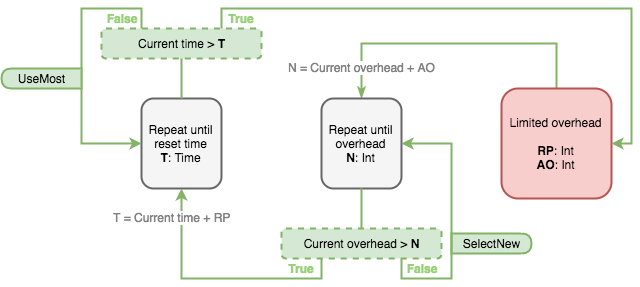
\includegraphics[width=85mm]{./img/limited_overhead.png}}}
	\caption{Transition diagram of the \textbf{Limited overhead} policy.}
	\label{fig:limited_overhead}
\end{figure}

Policies can be used to limit the library involvement per a real-time period, so that the selection overhead, or overhead generated by gathering data or wrongly selecting the slower function doesn't damage the system more than a specified limit. The \textbf{Limited overhead} policy in figure \ref{fig:limited_overhead} limits only the selection overhead time to \textit{AO} (allowed overhead) every \textit{RP} (reset period). After depleting the allowed time, it can't select anymore and keeps using the most selected function until the end of the period.

\begin{figure}[h!]
	\centerline{\mbox{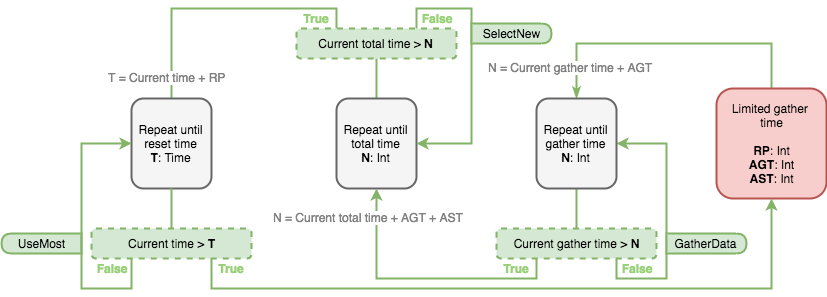
\includegraphics[width=85mm]{./img/limited_gather_time.png}}}
	\caption{Transition diagram of the \textbf{Limited gather time} policy.}
	\label{fig:limited_gather_time}
\end{figure}

In exactly the same way, the time spent on executing the function for the result GatherData and the whole process of selection and execution for the SelectNew result can be limited. The figure \ref{fig:limited_gather_time} demonstrates the \textbf{Limited gather time} policy, which keeps producing GatherData until total gather time reaches \textit{AGT} (allowed gather time), after that, it continues with the SelectNew result until total selection time reaches \textit{AST} (allowed selection time). A loop producing UseMost follows, for the rest of the real-time period specified by \textit{RP} (reset period).

This policy gives us control over the time spent on selecting results in real-time. If we get a lot of requests at the same time, receive a large batch of data to process or for any reason need to momentarily increase the throughput of the system, the time or overhead limits get depleted very quickly and the UseMost fallback result means reasonably good performance with a minimum overhead.

\subsection{Possible improvements}

Part of the statistical data could be a factor of combined certainty of all the selections of a specific function. This factor could be combined from the selection results of the strategies that would support it (in the statistical test based strategies, it could be a p-value, strength of the test, or similar) and would serve as a decision factor for more complex policies with a statistical approach as well.

The \textit{policies} were designed as a concept that is completely independent from the actual selection strategies and history analysis, to be faster and reusable. One of the improvements that would require closer tying would be to allow the \textit{policies} to choose the selection strategy, or to influence it somehow, by limiting it to a subset of data, etc. 

Another improvement that might seem useful is to allow the \textit{policies} to analyze the whole history data. This would, however, mean a lot of additional overhead time when evaluating the \textit{policy} and is not desirable.
With a different approach, we could achieve the same thing by giving selection strategies a state that could involve their decision. The state would be managed by the combined function and it could even be the same state that is used by the \textit{policies}. 

%TODO - when do I need more data?

\section{Grouping}

The problem with input dependency and with different expected decisions for various inputs can be partially solved by putting the history data and the function statistics according to the input into multiple groups. When deciding using the policies or selecting using one of the strategies described, only the data from the relevant group (based on the current input) is used. 

It would mean that the \textit{combined function} would need to hold the policy and the statistical data for every group, and the function run time history would have to be separate for different groups as well. The main advantage would be the possibility to take faster decisions in some groups, using for example the \textit{Pause selection after streak} policy. When a function is significantly faster than the others for very large inputs for example, it would quickly collect the streak for the decisions within the group, and the selection for future inputs from such a group would be quick.

\subsection{Group selection}

The group selection function that assigns an input into a group has to be provided by the user. The grouping can be based on the \textit{input descriptor}, but can also use other factors of the input, e.g., if there are some boolean flags passed to the function that affect its functionality, it is usually a good idea to use it in the grouping.

%TODO Reference to the policy

Some of the most common ways how to group values for the input descriptors might be:
\begin{itemize}
	\item Logarithmic - orders of magnitude
	\item Linear - tens, hundreds, thousands
	\item Fixed - predefined finite number of groups
\end{itemize}

The groups in general shouldn't be too small, as the selection process relies on only the data from the group. The advantage of groups with growing size (e.g. the logarithmic grouping) is that there is a lot of groups in the areas where the functions tend to compete in the performance (smaller inputs).